\documentclass[a4paper,11pt]{jsarticle}

% 数式
\usepackage{amsmath,amsfonts}
\usepackage{amsthm}
\usepackage{bm}
\usepackage{mathtools}

% 表
\usepackage[utf8]{inputenc}
\usepackage{diagbox} % 斜線付きセルを作成するために必要
\usepackage{booktabs} % 表の罫線を美しくするために必要
\usepackage{hhline} % 水平罫線を制御するために必要

% 画像
\usepackage[dvipdfmx]{graphicx}
\usepackage{ascmac}
\usepackage{physics}
\usepackage{float} % 追加

% 図
\usepackage[dvipdfmx]{graphicx}
\usepackage{tikz} %図を描く
\usetikzlibrary{positioning, intersections, calc, arrows.meta,math} %tikzのlibrary

% ハイパーリンク
\usepackage[dvipdfm,
  colorlinks=false,
  bookmarks=true,
  bookmarksnumbered=false,
  pdfborder={0 0 0},
  bookmarkstype=toc]{hyperref}

%式番号をセクション毎に
\numberwithin{equation}{section}

\begin{document}

\title{Lieb-Yngvasonノート}
\author{大上由人}
\date{\today}
\maketitle
\tableofcontents
\newpage
\section{状態と状態空間}
\subsection{状態と状態空間}
\begin{itembox}[l]{\textbf{Def:状態と状態空間}}
熱力学的状態は、状態空間$\Gamma$の点であり、$X,Y,Z$などと表す。
\end{itembox}
\textbf{ex}\\
温度$T_1$、体積$V_1$の状態を$(T,V) \in \Gamma$と表す。

\begin{itembox}[l]{\textbf{Def:状態空間の合成}}
    状態空間$\Gamma_1$と$\Gamma_2$の合成は、状態空間の直積$\Gamma_1 \times \Gamma_2$である。
\end{itembox}
\textbf{ex}\\
例えば、系1、系2をそれぞれ$(T_1,V_1),(T_2,V_2)$としたとき、それらをまとめて、$((T_1,V_1),(T_2,V_2))$

また、物理的直観から明らかなように、複数の状態空間を合成するとき、その合成の順序は問題にならない。すなわち、
\begin{equation}
    (\Gamma_1 \times \Gamma_2) \times \Gamma_3 = \Gamma_1 \times (\Gamma_2 \times \Gamma_3)
\end{equation}
である。

\subsection{スケーリングコピー}
\begin{itembox}[l]{\textbf{Def:スケーリングコピー}}
    $t>0$に対して、状態空間$\Gamma(t)$の構成要素を、$tX$とする。\\
    このとき、$\Gamma(t)$は、$\Gamma$のスケーリングコピーである。また、状態空間が$\mathbb{R}^n$の部分集合であるときは、$tX$は、ベクトルのスカラー倍としての表現となる。
    このとき、$\Gamma(t)=t\Gamma$と書く。
\end{itembox}
このとき、スケーリングコピーに関する以下の性質は、明らかである。
\begin{itemize}
    \item $\Gamma(1)=\Gamma$
    \item $1X=X$
    \item $(\Gamma(t))(s)=\Gamma(ts)$
    \item $s(tX)=(st)X$
    \item $(\Gamma_1 \times \Gamma_2)(t)=\Gamma_1(t) \times \Gamma_2(t)$
    \item $t(X,Y)=(tX,tY)$
\end{itemize}

\begin{itembox}[l]{\textbf{Def:多重スケーリングコピー}}
    状態空間が$\Gamma_1,\Gamma_2,\cdots,\Gamma_n$の直積であるとき、$t_1,t_2,\cdots,t_n>0$に対して、
    \begin{equation}
        \Gamma_1(t_1) \times \Gamma_2(t_2) \times \cdots \times \Gamma_n(t_n)
    \end{equation}
    なる直積を形成できる。とくに、$\Gamma_1=\Gamma_2=\cdots=\Gamma_n=\Gamma$のとき、
    \begin{equation}
        \Gamma(t_1,t_2,\cdots,t_n)=\Gamma(t_1) \times \Gamma(t_2) \times \cdots \times \Gamma(t_n)
    \end{equation}
    と書く。これを多重スケーリングコピーという
\end{itembox}

\textbf{ex:状態空間}\\
(a)水素が1molのとき、状態空間$\Gamma_a$は、エネルギーと体積で表され、$\mathbb{{R}}^2$の部分集合である。\\
(b)水素が0.5molのとき、状態空間$\Gamma_b$は、エネルギーと体積で表され、$\mathbb{{R}}^2$の部分集合であり、$\Gamma_b=\frac{1}{2}\Gamma_a=\{(\frac{1}{2}U,\frac{1}{2}V)|U,V \in \Gamma_a\}$である。\\
(c)水素が1mol、酸素が0.5mol(混合されていない)のとき、状態空間$\Gamma_c=\Gamma_a \times (酸素0.5molの状態空間)$であり、複合系である。\\
(d)水1molのとき、状態空間$\Gamma_d$\\
(e)水素1molと酸素0.5mol(混合)のとき、$\Gamma_e\neq \Gamma_d$であり、$\Gamma_e\neq \Gamma_c$である。\\

\newpage
\section{順序関係}
\subsection{断熱到達可能性}
状態空間の元に対して、順序関係を定める。
\begin{itembox}[l]{\textbf{Def:断熱到達可能性}}
    $X$から$Y$への状態変化が、外部装置\footnote{これは力学的仕事のみとは限らない。キャンセル法則の後を参照せよ。}とおもりとの相互作用によて可能であり、その過程で装置が初期状態に戻るとき\footnote{ただし、おもりは元の高さに戻らなくてよい。}、$X$から$Y$への断熱到達可能であるといい、
    \begin{equation}
        X \prec Y
    \end{equation}
    と書く。
    また、特に、$X$から$Y$への断熱到達可能であり、かつ、$Y$から$X$への断熱到達可能でないとき、
    \begin{equation}
        X \prec \prec Y
    \end{equation}
    と書く。
\end{itembox}
ただし、これは、いわゆる「断熱過程」を定義しているわけではない。\\

\textbf{ex:断熱到達可能性}\\
\begin{itemize}
    \item ガスの膨張または圧縮。これには、重りを持ち上げたり下げたりすることがあってもなくても含まれます。
    \item 擦ったりかき混ぜたりすること。
    \item 電気加熱。(ここでは「熱」という概念は必要ない。)
    \item ある障壁が取り除かれた後に孤立した複合システム内で発生する自然なプロセス。これには、混合や化学的、核反応が含まれる。
    \item ハンマーでシステムを破壊して分割し、再組み立てすること。
    \item このような変化の組み合わせ
\end{itemize}
これらは、すべて断熱到達可能である。(操作後に、外部装置が初期状態に戻ることが重要である。)\\

\begin{itembox}[l]{\textbf{Def:比較可能}}
    $X$と$Y$が比較可能であるとは、$X \prec Y$または$Y \prec X$であることをいう。
    また、両方の関係が成立するとき、$X$と$Y$は断熱的に等価であるといい、
    \begin{equation}
        X \overset{A}{\sim} Y
    \end{equation}
    と書く。

\end{itembox}
例えば、前の章で挙げた$(a)~(e)$の例はみな比較可能であり、また、(c)のすべての点が、(d)の多くの点と関係$\prec$で結ばれている。\\

\subsection{エントロピー原理}
以上の関係をもとに、後に示すエントロピー原理を書きなおす。
\begin{itembox}[l]{\textbf{エントロピー原理}}
    任意の状態$X$に対して、
    \begin{equation}
        X \prec Y \Leftrightarrow S(X) \leq S(Y)
    \end{equation}
    が成立する。
\end{itembox}
また、エントロピーの相加性や、示量性は以下のように書き直される。
\begin{itembox}[l]{\textbf{エントロピーの相加性}}
    $X$と$Y$が異なる系の状態であって、$(X,Y)$がそれらの合成系の状態であるとき、
    \begin{equation}
        S(X,Y)=S(X)+S(Y)
    \end{equation}
    が成立する。\\
    また、すべての$t>0$およびスケーリングコピー$tX$に対して、
    \begin{equation}
        S(tX)=tS(X)
    \end{equation}
    が成立する。
\end{itembox}
我々の目標は、これらを満たすエントロピーを公理から導き、なおかつそれが一意であることを示すことである。\\

\subsection{順序関係の公理}
\begin{itembox}[l]{\textbf{Axiom:順序関係の公理}}
    状態空間$\Gamma$上の順序関係$\prec$は、以下の公理を満たす。\\
    (A1: 反射律) $ X \overset{A}{\sim} X$\\
    (A2: 推移律) $X \prec Y$かつ$Y \prec Z$ならば、$X \prec Z$\\
    (A3: 一貫性) $X \prec X'$かつ$Y \prec Y'$ならば、$(X,Y) \prec (X',Y')$\\
    (A4: スケーリング不変性) $X \prec Y$ならば、$tX \prec tY$\\
    (A5: 分割と結合) $0<t<1$に対して、$X \overset{A}{\sim} (tX,(1-t)X)$\\
    (A6: 安定性) 0に近づく$\epsilon$の列およびいくつかの状態$Z_0,Z_1$に対して、$(X,\epsilon Z_0) \prec (Y,\epsilon Z_1)$ならば、$X \prec Y$ 
\end{itembox}
A3は、例えば断熱壁で隔てられた二つの系を考えたとき、合成系の壁をはずして片方の温度を下げることはできるが、逆は一般には不可能であることに対応している。\\
A6はぱっと見よくわからないが、要するに、外部系の微小な摂動が、状態の順序関係に影響を与えないことを述べている。\\
これらに加えて、比較仮説(CH)を導入する。これは、論文の後半で示されることとなる。\\
\begin{itembox}[l]{\textbf{Def:比較仮説}}
    状態空間に対してCHが成り立つとは、その空間内の任意の二つの状態$X$と$Y$が比較可能であることをいう。すなわち、
    \begin{equation}
        X \prec Y \quad or \quad Y \prec X \quad \forall X,Y \in \Gamma
    \end{equation}
    が成立することをいう。

\end{itembox}

\begin{itembox}[l]{\textbf{Thm:キャンセル法則}}
    $X,Y,Z$が系の状態のとき、
    \begin{equation}
        (X,Z) \prec (Y,Z) \Rightarrow X \prec Y
    \end{equation}
    が成立する。

\end{itembox}
\textbf{Prf}\\
$\epsilon =\frac{1}{n}$とする。このとき、
\begin{align}
    (X,\epsilon Z) &\overset{A}{\sim} ((1-\epsilon)X,\epsilon X,Z)\\
    &\prec ((1-\epsilon)X,\epsilon Y,Z)\\
    &\overset{A}{\sim} ((1-2\epsilon)X,\epsilon X,\epsilon Y,Z)\\
    &\prec ((1-2\epsilon)Y,2\epsilon Y,Z)
    \end{align}
これを$n=\frac{1}{\epsilon}$回繰り返すと、$X$の係数は0に、$Y$の係数は1に収束する。\\
以上より、$X \prec Y$が示された。\hfill\qedsymbol\\
この定理は、公理A3とは逆の方向の主張をしており、A3の制約がある中で、逆の主張がどの範囲まで成り立つかを示している。($X,Y$に対して同じ系を合成している。)

キャンセル法則のもとで、我々が定義した「断熱到達可能性」と、「断熱過程」が結びつくことを示す。\\
まず、断熱過程とは何であったかというと、「系が熱的に遮断された閉じた空間に閉じ込めらえれ、系への熱の流出入を防ぐ過程」のことであった。
したがって、系と外部との相互作用は、力学的または電磁気学的な仕事に限られる。\\
ここで、新たな記号$\prec ^*$を導入する。これは、$X$から$Y$への状態変化が、状態が$M$から$M'$に変化する外部装置が存在し、さらに、終状態において、何らかの方法でその装置を初期状態$M$に戻すことができるとき、$X$から$Y$への断熱到達可能であるということを表す。\\
すなわち、
\begin{equation}
    (X,M,h) \rightarrow (Y,M,h')
\end{equation}
が成立するとき、$X \prec ^* Y$と書く。\\
これは、「断熱過程」の定義と一致する。外部装置が熱の流出入を許していないことに注意されたい。\\

一方「断熱到達可能性」の定義では、外部装置にそのような制限はない。すなわち、外部装置は必要に応じて熱を生成したり、除去したりすることができる。\\
ただ、外部デバイスに対するそれ以外の制約は断熱過程の場合と同じである。すなわち、デバイスの状態を$D$で表すことにすると、
\begin{equation}
    (X,D,h) \rightarrow (Y,D,h')
\end{equation}
が成立するとき、$X \prec Y$である。\\

以上の議論を見ると、断熱過程は、断熱到達可能性の特殊な場合であることがわかる。すなわち、
\begin{equation}
    X \prec ^* Y \Rightarrow X \prec Y
\end{equation}
が成立する。\\
また、断熱到達可能性について、外部装置を力学的な部分と熱的な部分に分けると、$D = (M,Z)$と書ける。ここで、$M$は力学的な部分、$Z$は熱的な部分である。\\
このとき、
\begin{equation}
    (X,Z) \prec^* (Y,Z)
\end{equation}
であることがわかる。さらに、これにキャンセル法則を適応することができれば、
\begin{equation}
    X \prec^* Y
\end{equation}
が成立する。ただし、これに関しては正確な定義や証明はここでは行わない。(まず$\prec^*$の定義を明確にする必要がある。)\\
以上の議論をまとめると、
\begin{align}
    X \prec Y & \overset{def}{\Leftrightarrow} (X,M,Z,h) \prec (Y,M,Z,h')\\
    &\overset{def}{\Leftrightarrow} (X,Z) \prec^* (Y,Z)\\
    &\overset{?}{\Leftrightarrow} X \prec^* Y
\end{align}
となる。\\

\newpage
\section{エントロピーの構成}
\subsection{単純系}
今、状態空間$\Gamma$のスケールコピーを構成する。すなわち、
\begin{equation}
    Y =(t_1 Y_1,t_2 Y_2,\cdots,t_n Y_n) \quad (t_i>0), \quad Y_i \in \Gamma
\end{equation}
とする。\\
このとき、以下の命題が成り立つ。
\begin{itembox}[l]{\textbf{Prop:比較可能性}}
    $Y$が上のように書けるとき、同じように構成される$Y'$は、
    \begin{equation}
        Y' =(t_1' Y_1',t_2' Y_2',\cdots,t_m' Y_m') \quad t_j'>0, \quad Y_j' \in \Gamma
    \end{equation}
    であるとする。また、
    \begin{equation}
        \sum_{i=1}^n t_i = \sum_{j=1}^m t_j'
    \end{equation}
    であるとする。このとき、$Y$と$Y'$は比較可能である。
\end{itembox}
\textbf{Prf}\\
特に、$n=m=2$の場合を考える。このとき、
\begin{equation}
    t_1-t_1' = t_2'-t_2
\end{equation}
である。$t_1-t_1' =0$のとき、
\begin{align}
    Y &= (t_1 Y_1,t_2 Y_2)\\
    Y' &= (t_1 Y_1',t_2 Y_2')
\end{align}
であるから、$Y$と$Y'$はともに$\Gamma _{t_1} \times \Gamma _{t_2}$の点であり、比較可能である。\\
また、$t_1-t_1' >0$のとき、A5より、
\begin{align}
    Y=(t_1 Y_1,t_2 Y_2) &\overset{A}{\sim} (t_1' Y_1,(t_1-t_1')Y_1,t_2 Y_2)\\
    Y'=(t_1' Y_1',t_2 Y_2') &\overset{A}{\sim} (t_1' Y_1',(t_2'-t_2)Y_2',t_2 Y_2')=(t_1' Y_1',(t_1-t_1')Y_2',t_2 Y_2')
\end{align}
であるから、$Y$と$Y'$はともに、$\Gamma _{t_1} \times \Gamma _{t_1-t_1'} \times \Gamma _{t_2}$の点であり、比較可能である。\\
以上より、一般の場合についても、$Y$と$Y'$は比較可能である。\hfill\qedsymbol\\
この定理のもと、単純系の多重スケーリングコピーにおいてエントロピー原理を導出することができる。\\
\begin{itembox}[l]{\textbf{Thm:エントロピー(単純系)}}
    以下の(1),(2)は同値である。\\
    (1) 関係$\prec$が、$\Gamma$の多重スケーリングコピーにおいて、順序の公理A1-A6及び比較仮説(CH)を満たす。\\
    (2) ある関数$S_{\Gamma}:\Gamma \rightarrow \mathbb{R}$が存在して、以下の性質を満たす。\\
    もし、$(t_1+ \cdots +t_n)=t_1'+ \cdots +t_m'$であるとき、
    \begin{equation}
        (t_1 Y_1, \cdots ,t_n Y_n) \prec (t_1' Y_1', \cdots ,t_m' Y_m') \Leftrightarrow S_{\Gamma}(Y_1)+ \cdots +S_{\Gamma}(Y_n) \leq S_{\Gamma}(Y_1')+ \cdots +S_{\Gamma}(Y_m')
    \end{equation}
    が成立する。\\
    また、この関数は、アフィン変換を除いて、$\Gamma$に対して一意に定まる。

\end{itembox}
いくらかの補題を証明しておく。\\
\begin{itembox}[l]{\textbf{Lem2.1}}
$X_0,X_1$が状態空間$\Gamma$の点で、$X_0 \prec \prec X_1$であるとする。このとき、実数$\lambda$に対して、
\begin{equation}
    \mathcal{S}_{\lambda} = \{X\in \Gamma|((1-\lambda)X_0,\lambda X_1) \prec X \}
\end{equation}
と定義する。このとき、以下の二つの主張が成立する。\\
(1) 任意の$X \in \Gamma$に対して、$X \in \mathcal{S}_{\lambda}$となるような$\lambda$が存在する。\\
(2) 任意の$X \in \Gamma$に対して、$\sup\{\lambda|X \in \mathcal{S}_{\lambda}\}<\infty$である。

\end{itembox}
この補題は、カノニカルエントロピーがwell-definedであることおよび、有限であることを示している。\\
\textbf{Prf}\\
(1) \\
$X_0 \prec X$であるとき、A2より、明らかに$X \in \mathcal{S}_0$である。\\
一般の$X$について示す。ここで、$\alpha \geq 0$に対して、
\begin{equation}
    (1+\alpha)X_0 \prec (\alpha X_1,X)
\end{equation}
が成り立つことを示す。もしこれが成り立たないとすると、CHより、
\begin{equation}
    (\alpha X_1,X) \prec (1+\alpha)X_0
\end{equation}
が成立する。このとき、
\begin{align}
    (X_1,\frac{1}{\alpha}X) &\prec \frac{\alpha+1}{\alpha}(\frac{1}{1+\alpha}X_0+\frac{\alpha}{1+\alpha}X_0)\\
    \frac{\alpha}{\alpha+1}(X_1,\frac{1}{\alpha}X) &\prec (\frac{1}{1+\alpha}X_0+\frac{\alpha}{1+\alpha}X_0)\\
    &\overset{A}{\sim} (\frac{1}{1+\alpha}X_0,\frac{\alpha}{1+\alpha}X_0)\\
\end{align}
であるから、
\begin{align}
    (X_1,\frac{1}{\alpha}X) &\prec (X_0,\frac{1}{\alpha}X_0)
\end{align}
がいえる。これと、A6(安定性)より、$X_1 \prec X_0$である。これは、$X_0 \prec \prec X_1$に矛盾する。\\
以上より、(30)式が示された。ここで、$\alpha = -\lambda$とすると、
\begin{equation}
    (1-\lambda)X_0 \prec (-\lambda X_1,X)
\end{equation}
これの両辺に$\lambda X_1$を加えると、
\begin{equation}
    (1-\lambda)X_0 + \lambda X_1 \prec X
\end{equation}
であるから、$X \in \mathcal{S}_{\lambda}$である。\\
(2)\\
背理法により示す。$sup\{\lambda|X \in \mathcal{S}_{\lambda}\}=\infty$であるとする。このとき、$X\in \mathcal{S}_{\lambda}$について、
\begin{equation}
    ((1-\lambda)X_0,\lambda X_1) \prec X
\end{equation}
である。これを変形して、
\begin{equation}
    (X_0,\lambda X_1) \prec (\lambda X_0,X)
\end{equation}
スケーリング不変性より、
\begin{equation}
    (X_1,\frac{1}{\lambda}X_0) \prec (X_0,\frac{1}{\lambda}X)
\end{equation}  
ここで、$\lambda \rightarrow \infty$として、キャンセル法則を用いることにより、
\begin{equation}
    X_1 \prec X_0
\end{equation}
がいえる。これは、$X_0 \prec \prec X_1$に矛盾する。\\
以上より、(2)が示された。\hfill\qedsymbol\\

\begin{itembox}[l]{\textbf{Def:カノニカルエントロピー/基準点}}
    状態空間$\Gamma$上のある$X_0,X_1$に対して、$X_0 \prec \prec X_1$であるとする。このとき、
    \begin{equation}
        S_{\Gamma}(X) = \sup\{\lambda|((1-\lambda)X_0,\lambda X_1) \prec X\}
    \end{equation}
    で定義される関数$S_{\Gamma}$を、基準点$X_0 \prec \prec X_1$に関するカノニカルエントロピーという。\\
    また、カノニカルエントロピーは、
    \begin{equation}
        S_{\Gamma}(X) = \sup\{\lambda|X \in \mathcal{S}_{\lambda}\}
    \end{equation}
    とも書ける。
\end{itembox}
基準点を設ける意味は、もし、系のすべてが断熱的に等価であるならば、状態空間にわたってエントロピーが一定となるからである。\\


\begin{figure}[H]
    \begin{center}
    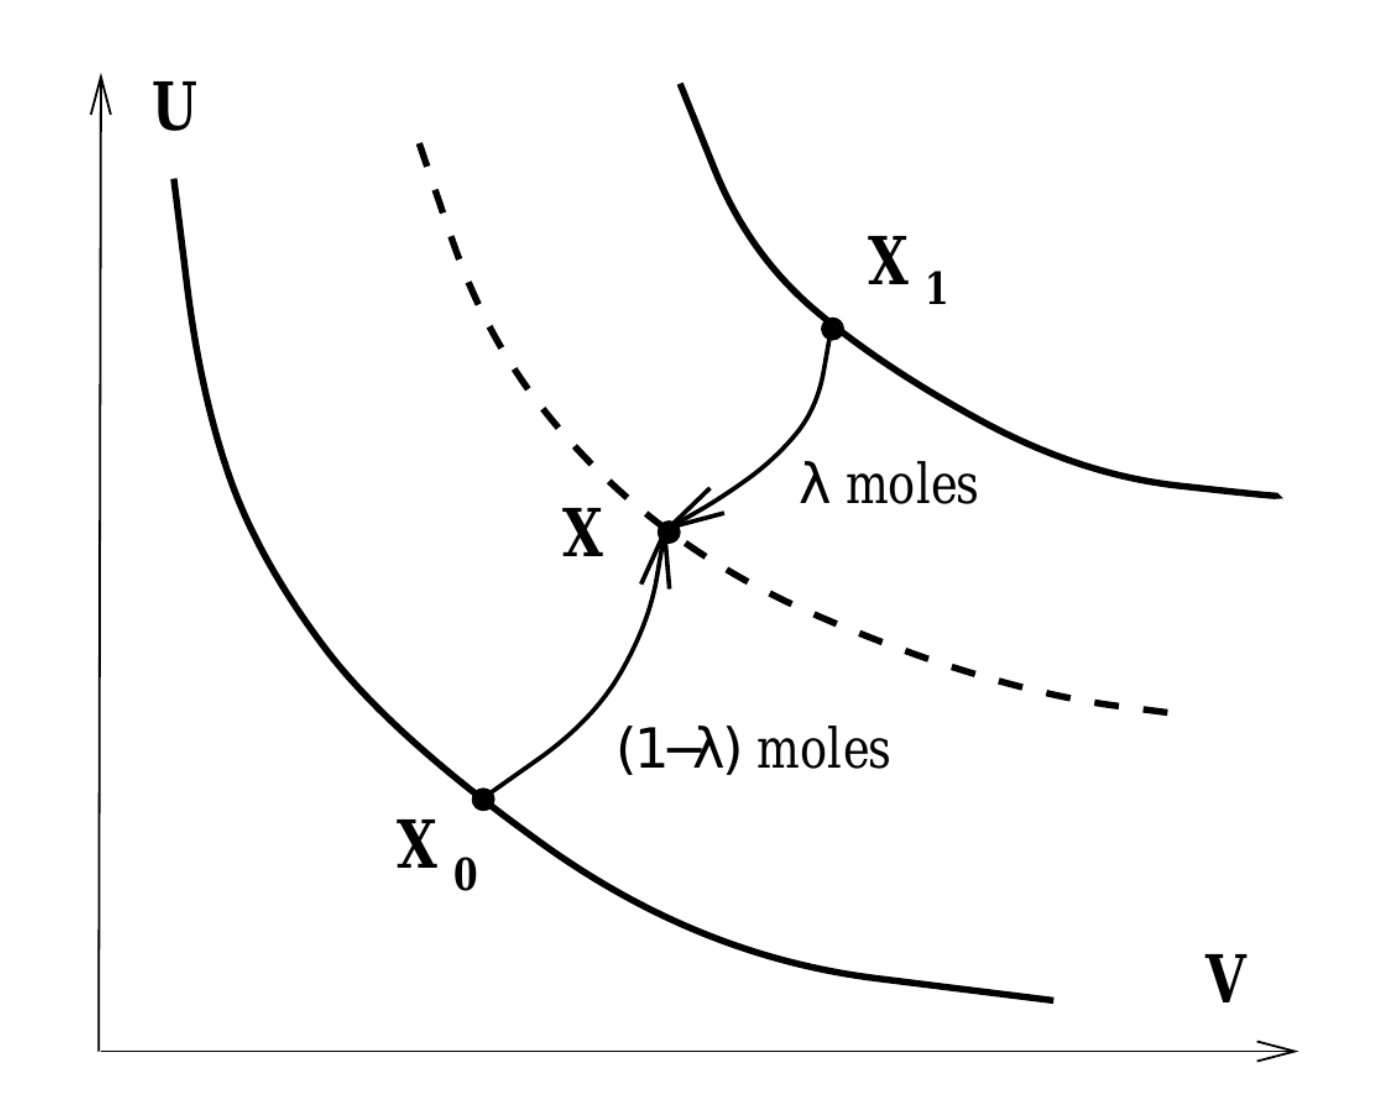
\includegraphics[width=50mm]{fig2.png}
    \end{center}
    \caption{カノニカルエントロピー}
    \label{fig:one}
\end{figure}
Lemma2.1により、カノニカルエントロピーは、well-definedであり、$S_{\Gamma}(X)<\infty$である。\\

\begin{itembox}[l]{\textbf{Lem2.2:$\prec$と$\leq$の関係}}
    いま、$X_0 \prec \prec X_1$であるとし、$a_0,a_1,a_0',a_1' \in \mathbb{R}$に対して、$a_0+a_1=a_0'+a_1'$であるとする。このとき、\\
    (1)$((a_0X_0,a_1X_1) \prec (a_0'X_0,a_1'X_1))$\\
    (2)$ a_1 \leq a_1' $(ゆえに、$a_0 \leq a_0'$)\\
    は同値である。\\
    特に、もし、$a_1=a_1',a_0=a_0'$であるならば、(1)の$\prec$は$\overset{A}{\sim}$に置き換えることができる。
\end{itembox}
これは、例えば、温度の高い系と低い系を接触させたときに、エントロピーが増加することを示している。\\
\textbf{Prf}\\
ここでは、$a_0,a_1,a_0',a_1'$が全て正であり、$a_0+a_1=a_0'+a_1'=1$であるとする。また、$a_1=\lambda,a_1'=\lambda'$とする。\\
(1)$\Rightarrow$(2)\\
背理法により示す。すなわち、$\lambda > \lambda'$とする。今、
\begin{equation}
    ((1-\lambda)X_0,\lambda X_1) \prec ((1-\lambda')X_0',\lambda'X_1')
\end{equation}
ここで、
\begin{align}
    ((1-\lambda)X_0,\lambda X_1) &\overset{A}{\sim} ((1-\lambda)X_0,\lambda'X_1,(\lambda-\lambda')X_1)\\
    ((1-\lambda')X_0,\lambda'X_1') &\overset{A}{\sim} ((1-\lambda)X_0,(\lambda - \lambda')X_0,\lambda'X_1)
\end{align}
であるから、
\begin{equation}
    ((1-\lambda)X_0,\lambda'X_1,(\lambda-\lambda')X_1) \prec ((1-\lambda)X_0,(\lambda - \lambda')X_0,\lambda'X_1)
\end{equation}
である。ここで、キャンセル法則を用いると、
\begin{equation}
    (\lambda - \lambda')X_1 \prec (\lambda - \lambda')X_0
\end{equation}
$\lambda -\lambda '>0$と、スケーリング不変性より、
\begin{equation}
    X_1 \prec X_0
\end{equation}
であるが、これは、$X_0 \prec \prec X_1$に矛盾する。\\
(2)$\Rightarrow$(1)\\
\begin{align}
    ((1-\lambda)X_0,\lambda X_1) &\overset{A}{\sim} ((1-\lambda')X_0,(\lambda'-\lambda)X_0,\lambda X_1)\\
    &\prec ((1-\lambda')X_0,(\lambda'-\lambda)X_1,\lambda X_1)\\
    &\overset{A}{\sim} ((1-\lambda')X_0,\lambda'X_1)
\end{align}
であるから、(1)が示された。 \hfill\qedsymbol\\


\begin{itembox}[l]{\textbf{Lem2.3:エントロピーの特徴づけ}}
$S_{\Gamma}$が、$\Gamma$上のカノニカルエントロピーであるとし、基準点を$X_0 \prec \prec X_1$とする。もし、$X\in \Gamma$であるならば、
\begin{equation}
    \lambda = S_{\Gamma}(X)
\end{equation}
は、
\begin{equation}
    X \overset{A}{\sim} ((1-\lambda)X_0,\lambda X_1)
\end{equation}
と同値である。\\

\end{itembox}
\textbf{Prf}\\
((53)$\Rightarrow$(54))\\
$\lambda = S_{\Gamma}(X)$とする。このとき、supの定義より、0に収束する列$\epsilon_n$の列が存在して、
\begin{equation}
    ((1-(\lambda-\epsilon_n))X_0,(\lambda-\epsilon_n)X_1) \prec X
\end{equation}
である。任意のnについて、
\begin{align}
    ((1-\lambda)X_0,\lambda X_1,\epsilon_n X_0) &\overset{A}{\sim} ((1-(\lambda+\epsilon_n))X_0,(\lambda-\epsilon_n)X_1,\epsilon_n X_1)\\
    &\prec (X,\epsilon_n X_1)
\end{align}
である。安定性を用いて、
\begin{equation}
    ((1-\lambda)X_0,\lambda X_1) \prec X
\end{equation}
である。\\
また、$\lambda$はsupなので、
\begin{equation}
    X \prec ((1-(\lambda+\epsilon))X_0,(\lambda+\epsilon)X_1)
\end{equation}
である。変形して、
\begin{equation}
    X+\epsilon X_0 \prec ((1-\lambda)X_0,\lambda X_1)
\end{equation}
である。ここで、安定性を用いて、
\begin{equation}
    X \prec ((1-\lambda)X_0,\lambda X_1)
\end{equation}
以上より、
\begin{equation}
    X \overset{A}{\sim} ((1-\lambda)X_0,\lambda X_1)
\end{equation}
である。 \\

((54)$\Rightarrow$(53))\\

\textbf{Prf(Thm2.2)}\\
((1)$\Rightarrow$(2))\\
$\lambda_i = S_{\Gamma}(Y_i)$とする。このとき、Lem2.3より、
\begin{align}
    Y_i \overset{A}{\sim} (1-S_{\Gamma}(Y_i))X_0,S_{\Gamma}(Y_i)X_1\\
    Y_i' \overset{A}{\sim} (1-S_{\Gamma}(Y_i'))X_0,S_{\Gamma}(Y_i')X_1
\end{align}
である。これより、
\begin{align}
    (t_1 Y_1,t_2 Y_2,\cdots,t_n Y_n) &\overset{A}{\sim} (\sum_{i=1}^n t_i(1-S_{\Gamma}(Y_i))X_0,\sum_{i=1}^n t_i S_{\Gamma}(Y_i)X_1)\\
    (t_1' Y_1',t_2' Y_2',\cdots,t_n' Y_n') &\overset{A}{\sim} (\sum_{i=1}^n t_i'(1-S_{\Gamma}(Y_i'))X_0,\sum_{i=1}^n t_i' S_{\Gamma}(Y_i')X_1)
\end{align}
である。ここで、右辺について、Lem2.2より、
\begin{equation}
    \sum_{i=1}^n t_i S_{\Gamma}(Y_i) \leq \sum_{i=1}^n t_i' S_{\Gamma}(Y_i')
\end{equation}
である。\\
((2)$\Rightarrow$(1))\\
略。(要するに、普段扱っているエントロピーが自然な仮説$A_1-A_6$およびCHを満たすか確かめる作業である。)\\
以上より、示された。\hfill\qedsymbol\\

\begin{itembox}[l]{\textbf{Thm:エントロピーの一意性}}
もし、$S_{\Gamma}^*$が、任意の$\lambda \in \mathbb{R}$と、$X,Y,X',Y' \in \Gamma $に対して、
\begin{align}
    ((1-\lambda)X,\lambda Y) &\prec ((1-\lambda')X',\lambda' Y') \\
    \Leftrightarrow (1-\lambda)S_{\Gamma}^*(X)+\lambda S_{\Gamma}^*(Y) &\leq (1-\lambda')S_{\Gamma}^*(X')+\lambda' S_{\Gamma}^*(Y')
\end{align}
であるならば、
\begin{equation}
    S_{\Gamma}^*(X)=aS_{\Gamma} (X)+b
\end{equation}
で表される。ただし、
\begin{align}
    a = S_{\Gamma}^*(X_1)-S_{\Gamma}^*(X_0)>0\\
    b = S_{\Gamma}^*(X_0)
\end{align}
である。\\
ここで、$S_{\Gamma}$は、$\Gamma$上のカノニカルエントロピーで、参照点は$X_0 \prec \prec X_1$である。
\end{itembox}
\textbf{Prf}\\
Lem2.3より、
\begin{equation}
    X \overset{A}{\sim} ((1-\lambda)X,\lambda X) \overset{A}{\sim} ((1-\lambda')X_0,\lambda' X_1)
\end{equation}
である。$S_{\Gamma}^*$に関する仮定(Thm2.2)より、
\begin{equation}
    S_{\Gamma}^*(X) = (1-\lambda')S_{\Gamma}^*(X_0)+\lambda' S_{\Gamma}^*(X_1)=(S_{\Gamma}^*(X_1)-S_{\Gamma}^*(X_0))\lambda'+S_{\Gamma}^*(X_0)
\end{equation}
ここで、$X \overset{A}{\sim} ((1-\lambda')X_0,\lambda' X_1)$であるから、Lem2.3より、$\lambda ' = S_{\Gamma}(X)$である。\\
以上より、
\begin{equation}
    S_{\Gamma}^*(X) = aS_{\Gamma}(X)+b
\end{equation}
である。\hfill\qedsymbol\\

カノニカルエントロピーの定義をみてみると、エントロピーは、二重スケール積$\Gamma(1-\lambda)\times \Gamma(\lambda)$上の関係$\prec$と、基準点$X_0 \prec \prec X_1$のみに依存している。\\
さらに、Thm2.2の(2)$ \Rightarrow $(1)に注目すると、エントロピーは、すべての多重スケーリングコピーにおいて、順序関係を定め、CHを満たす。\\

\begin{itembox}[l]{\textbf{Thm:エントロピーの一意性(2)}}
    $\prec$と$\prec ^*$を、$\Gamma$上のスケールコピーにおける関係とし、公理A1-A6を満たし、さらに、固定された各$\lambda \in [0,1]$について、$\Gamma(1-\lambda)\times \Gamma(\lambda)$についてCHも満たすとする。\\
    もし、$\prec$と$\prec ^*$が[0,1]の各$\lambda\in [0,1]$について、$\Gamma(1-\lambda)\times \Gamma(\lambda)$上で一致しているならば、$\prec$と$\prec ^*$は$\Gamma$のすべての複数スケールコピー上で一致し、CHはすべての複数スケールコピーにおいて成立する。
\end{itembox}

\subsection{混合のない複合系}
\begin{itembox}[l]{\textbf{Def:エントロピー定数}}
    Thm2.3における$a,b$を、エントロピー定数という。
\end{itembox}
我々の目標は、これらのエントロピーをまとめて、さまざまな系の任意の多重スケーリングコピー積に対して正しく振舞うことを示すことである。\\
また、この普遍的エントロピーは、系ごとに乗法定数が一意に定まる。\\
ここでの問題は、キャリブレーションである。すなわち、各基本エントロピーの前にある乗法定数を、(2.4)が守られるように選択する必要がある。\\
このsectionでは、以下の定理を証明する。これは、Thm2.2の一般化である。\\

\begin{itembox}[l]{\textbf{Thm:Consistent entropy scales}}
以下の要件を満たす系からなる族(SF)を考える。\\
\begin{itemize}
    \item[(1)] SFの任意の二つの系の状態空間は互いに素な集合である。すなわち、SF内のすべての状態はちょうど一つの状態空間に属する。\\
    \item[(2)] SF内の任意の多重スケーリング積もまたSFに属する。\footnote{ただし、例えば$\Gamma_1 \times \Gamma_2$は$\Gamma_1$や$\Gamma_2$と互いに素である。}\\
    \item[(3)] SF内の任意の系がCHを満たす。\\
\end{itemize}
それぞれの状態空間$\Gamma$に対して、$S_{\Gamma}$を$\Gamma$上ある確定されたエントロピー関数とする。このとき、$\Gamma$のすべての状態に対して定義される関数
\begin{equation}
    S(X) = a_{\Gamma}S_{\Gamma}(X)+b_{\Gamma} \quad X \in \Gamma
\end{equation}
が、以下の性質を持つ。\\
\begin{itemize}
    \item[(a)] もし、$X$と$Y$が同じ状態空間に属するならば、$X \prec Y \Leftrightarrow S(X) \leq S(Y)$である。\\
    \item[(b)] $S$は相加性と示量性を持つ。すなわち、
    \begin{align}
        S(X,Y) &= S(X)+S(Y)\\
        S(tX) &= tS(X)
    \end{align}
    である。\\
\end{itemize}
\end{itembox}
\textbf{Prf}\\
ある系$\Gamma_0$と、$\Gamma_0$上の二点$Z_0 \prec \prec Z_1$を選ぶ。それのれの状態空間に対して、ある固定点$X_{\Gamma}\in \Gamma$を、
\begin{align}
    X_{\Gamma_1 \times \Gamma_2} &= (X_{\Gamma_1},X_{\Gamma_2})\\
    X_{t\Gamma} &= tX_{\Gamma}
\end{align}
が成り立つように選ぶ。\\
中略\\
$X \in \Gamma$に対して、$\Gamma \times \Gamma_0$とその空間上の、基準点が$(X_{\Gamma},Z_0),(X_{\Gamma},Z_1)$であるようなカノニカルエントロピーを考える。このとき、新たにエントロピー関数を、
\begin{equation}
    S(X)=S_{\Gamma_1 \times \Gamma_2}((X,Z_0)|(X_{\Gamma},Z_0),(X_{\Gamma},Z_1))
\end{equation}
と定義する。\\
このように定義すると、合成系について、Le.2.3を適用することで、
\begin{equation}
    (X,Z_0) \overset{A}{\sim} ((1-\lambda)(X_{\Gamma},Z_0),\lambda(X_{\Gamma},Z_1))
\end{equation}
である。ただし、$\lambda = S(X)$である。これを変形することにより、
\begin{equation}
    (X,\lambda Z_0) \overset{A}{\sim} (X_{\Gamma},\lambda Z_1)
\end{equation}
である。この(83)式を整理することで、エントロピーの加法性を示すことができる。\\
\textbf{加法性}\\
\begin{align}
    (X_1,\lambda_1 Z_0) &\overset{A}{\sim} (X_{\Gamma_1},\lambda_1 Z_1)\\
    (X_2,\lambda_2 Z_0) &\overset{A}{\sim} (X_{\Gamma_2},\lambda_2 Z_1)\\
    (X,\lambda Z_0) &\overset{A}{\sim} (X_{\Gamma},\lambda Z_1)
\end{align}
である。上二つの式から、
\begin{align}
    ((X_1,\lambda_1 Z_0),(X_2,\lambda_2 Z_0)) &\overset{A}{\sim} ((X_{\Gamma_1},\lambda_1 Z_1),(X_{\Gamma_2},\lambda_2 Z_1))\\
    &\overset{A}{\sim} (X_{\Gamma_1},X_{\Gamma_2},(\lambda_1+\lambda_2)Z_1)
\end{align}
である。これと(86)式を比較して、
\begin{equation}
    S(X_1)+S(X_2) = S(X_1,X_2)
\end{equation}
である。\\
\textbf{示量性}\\
\begin{align}
    (X,\lambda Z_0) &\overset{A}{\sim} (X_{\Gamma},\lambda Z_1)\\
    (tX,\lambda' Z_0) &\overset{A}{\sim} (X_{t\Gamma},\lambda' Z_1)=(tX_{\Gamma},\lambda' Z_1)\\
    (tX,\lambda' Z_0) &\overset{A}{\sim} (X_{\Gamma},\frac{\lambda'}{t} Z_1)
\end{align}
であるから、
\begin{equation}
    \lambda = \frac{\lambda'}{t}
\end{equation}
であるから、$S(tX)=tS(X)$である。\\
また、これがエントロピーとしての資格を持つことは、以下のように示すことができる。\\
\textbf{エントロピー増大則}\\
\begin{equation}
    X \prec Y \Leftrightarrow S(X) \leq S(Y)
\end{equation}
を示す。キャンセル法則を用いることにより、
\begin{equation}
    X \prec Y \Leftrightarrow (X,Z_0) \prec (Y,Z_0)
\end{equation}
を示す。キャンセル法則を用いることにより、
\begin{equation}
    X \prec Y \Leftarrow (X,Z_0) \prec (Y,Z_0)
\end{equation}
である。また、Thm2.2により、
\begin{equation}
    (X,Z_0) \prec (Y,Z_0) \Leftrightarrow S(X,Z_0) \leq S(Y,Z_0) \Leftrightarrow S(X) \leq S(Y)
\end{equation}
であるから、エントロピー増大則が示された。\hfill\qedsymbol\\

\begin{itembox}[l]{\textbf{Def:一貫したエントロピー}}
    状態空間$\Gamma$上のエントロピー関数$S_{\Gamma}$が一貫したエントロピーであるとは、$\Gamma$上のエントロピー関数の適切な線形結合が、任意の多重スケーリング積のエントロピー関数として働くことである。\\
    すなわち、すべての多重スケーリングコピーにおいて$a_{\Gamma}$を1にとることができるということである。
\end{itembox}
要するに、エントロピーの目盛りを合わせることができるということである。例えば、上の証明で構成したエントロピーは、任意の状態についてエントロピーの係数を1にとることができている。\\

以上のエントロピーの議論により、我々は、適当な状態空間(これは複数の単純系のスケールコピーでもよい)上の状態について、エントロピーを定義することができ、また、そのエントロピーのは、単純系で定義したものと同じ尺度ではかることができるということがわかった。\\

\textbf{注意}\\
エントロピー関数は、
\begin{equation}
    S(X) =\text{sup}\{\lambda|(X_{\Gamma},\lambda Z_1)\prec (X,\lambda Z_0)\}
\end{equation}
とも書くことができる。\\

\subsection{エントロピーの凸性}
\begin{itembox}[l]{\textbf{Def:凸な状態空間}}
    状態空間$\Gamma$が凸であるとは、任意の$X,Y \in \Gamma$について、
    \begin{equation}
        (tX+(1-t)Y) \in \Gamma \quad (0 \leq t \leq 1)
    \end{equation}
    が成立することである。
\end{itembox}

さて、以上の定義のもと、断熱到達可能性に、以下の公理を追加する。\\
\begin{itembox}[l]{\textbf{順序関係の公理A7}}
    状態空間$\Gamma$が凸であるとし、$X,Y \in \Gamma$であるとする。このとき、
    \begin{equation}
        (tX,(1-t)Y) \prec tX+(1-t)Y
    \end{equation}
    が成立する。
\end{itembox}
この要請の物理的要請は、独立した二つの系を合成したとき、例えばエネルギーや体積が加算されることを意味する。

\begin{itembox}[l]{\textbf{Def:forward sector}}
    状態空間$\Gamma,\Gamma'$と、$X \in \Gamma,Y \in \Gamma'$に対して、
    \begin{equation}
        A_X = \{Y \in \Gamma'|X \prec Y\}
    \end{equation}
    を、$X$のforward sectorという。
\end{itembox}
\begin{itembox}[l]{\textbf{Thm:forward sectorの凸性}}
    $\Gamma,\Gamma'$を状態空間とし、$\Gamma '$が凸であるとする。このとき、$X \in \Gamma$に対して、$A_X$は$\Gamma'$の凸集合である。
\end{itembox}
\textbf{Prf}\\
$X \prec Y_1,Y_2$であるとし、$0 < t < 1$とする。このとき、
\begin{align}
    X \prec tY_1+(1-t)Y_2
\end{align}
を示せばよい。A5より、
\begin{equation}
    X \prec (tX,(1-t)X)
\end{equation}
である。また、$X \prec Y_1,Y_2$であるから、
\begin{align}
    (tX,(1-t)X) \prec (tY_1,(1-t)Y_2)
\end{align}
である。これと、A7より、
\begin{equation}
    X \prec tY_1+(1-t)Y_2
\end{equation}
である。以上より、示された。\hfill\qedsymbol\\
とくに、同じ状態空間内でのA7と上の定理を図示すると、以下のようになる。\\
\begin{figure}[H]
    \begin{center}
    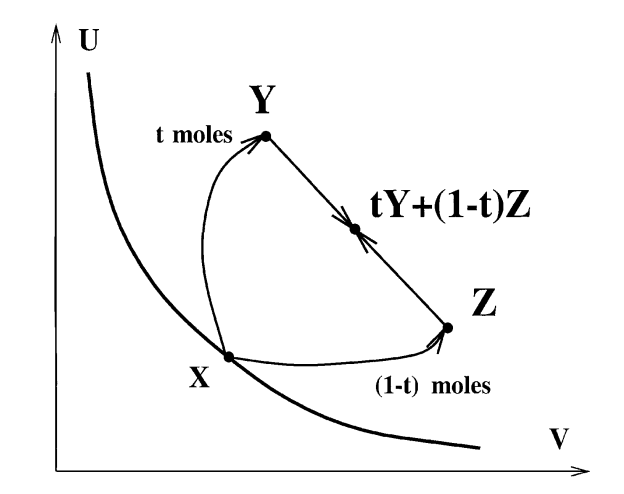
\includegraphics[width=100mm]{fig3.png}
    \end{center}
    \caption{forward sector}
    \label{fig:two}
\end{figure}
すなわち、断熱到達可能なYとZが存在するとき、YとZの間には、さらに断熱到達可能な点が存在するということである。\\

\begin{itembox}[l]{\textbf{Thm:$\mathcal{S}_{\lambda}$の凸性}}
    状態空間$\Gamma$が凸であるとき、以下の二つが成立する。
    \begin{itemize}
        \item[(1)] $\mathcal{S}_{\lambda}$は、$\Gamma$の凸集合である。
        \item[(2)] もし、$X \in \mathcal{S}_{\lambda}$であり、$0 \leq t \leq 1$であるならば、$tX + (1-t)Y \in \mathcal{S}_{t\lambda \times (1-t)\lambda}$である。
    \end{itemize}
\end{itembox}
\textbf{Recall}\\
$\mathcal{S}_{\lambda}= \{X \in \Gamma|((1-\lambda)X_0,\lambda X_1) \prec X\}$である。\\
\textbf{Prf}\\
(1)\\
$X,Y \in \mathcal{S}_{\lambda}$であるとする。このとき、
\begin{align}
    tX+(1-t)Y \in \mathcal{S}_{\lambda}
\end{align}
を示せばよい。ここで、$X,Y \in \mathcal{S}_{\lambda}$であるから、
\begin{align}
    ((1-\lambda)X_0,\lambda X_1) &\prec X\\
    ((1-\lambda)X_0,\lambda X_1) &\prec Y
\end{align}
である。したがって、
\begin{align}
    t((1-\lambda)X_0,\lambda X_1) &\prec tX\\
    (1-t)((1-\lambda)X_0,\lambda X_1) &\prec (1-t)Y
\end{align}
である。したがって、
\begin{align}
    t((1-\lambda)X_0,\lambda X_1)+(1-t)((1-\lambda)X_0,\lambda X_1) &\prec tX+(1-t)Y\\
    ((1-\lambda)X_0,\lambda X_1) &\prec tX+(1-t)Y
\end{align}
である。以上より、(1)が示された。\\
(2)\\
後で書く。\\

\begin{itembox}[l]{\textbf{Thm:エントロピーの凸性}}
    状態空間$\Gamma$が凸であるとする。このとき、エントロピー関数$S_{\Gamma}$は、
    \begin{equation}
        S_{\Gamma}(tX+(1-t)Y) \geq tS_{\Gamma}(X)+(1-t)S_{\Gamma}(Y)
    \end{equation}
    である。すなわち、$S_{\Gamma}$は、上に凸である。
\end{itembox}
\textbf{Prf}\\
$X \in \mathcal{S}_{\lambda_1},Y \in \mathcal{S}_{\lambda_2}$であるとする。このとき、Thm2.7より、
\begin{align}
    tX+(1-t)Y \in \mathcal{S}_{t\lambda_1+(1-t)\lambda_2}
\end{align}
である。このとき、エントロピーの定義から、
\begin{align}
    S_{\Gamma}(tX+(1-t)Y) &\geq t\lambda_1+(1-t)\lambda_2\\
\end{align}
である。したがって、右辺の$\lambda_1,\lambda_2$についてsupを取ることにより、
\begin{align}
    S_{\Gamma}(tX+(1-t)Y) &\geq tS_{\Gamma}(X)+(1-t)S_{\Gamma}(Y)
\end{align}
である。以上より、示された。\hfill\qedsymbol\\

\subsection{不可逆過程とカラテオドリの原理}
\begin{itembox}[l]{\textbf{Thm:カラテオドリの原理と不可逆過程}}
    状態空間$\Gamma$が凸であり、$\mathbb{R}^n$の部分空間であるとする。このとき、以下の二つの主張を考える。
    \begin{itemize}
        \item[(1)] 不可逆過程の存在:任意の$X \in \Gamma$に対して、$X \prec \prec Y$となる$Y \in \Gamma$が存在する。
        \item[(2)] カラテオドリの原理:任意の$X \in \Gamma$の任意の近傍にたいして、$Z \overset{A}{\sim} X$が偽となる$Z \in \Gamma$が存在する。 
    \end{itemize}
    このとき、(1)$\Rightarrow$(2)である。\\
また、$\Gamma$上の任意のforward sectorが、成分0をもたないならば、(2)$\Rightarrow$(1)である。
\end{itembox}
\textbf{Prf}\\
一旦省略\\

\newpage
\section{単純系}
単純系の取り扱いについて考える。
\begin{itembox}[l]{\textbf{Def:単純系/複合系}}
ある系が単純系であるとは、系の状態が、一つのエネルギー座標とその他の仕事座標(体積など)によって特徴づけられるときである。\\
一方、複合系とは、系の状態が、複数のエネルギー座標によって特徴づけられるときである。
\end{itembox}

以下(単純系に限らず)考えるすべての系は、単純系のスケーリング積によって構成される。\\
単純系と単純系でないものの例を挙げると以下のようになる。\\
\textbf{単純系}
\begin{itemize}
    \item[(1)] 1molの水が入ったピストン付き容器(仕事座標は体積)
    \item[(2)] ピストン付き容器に入った0.5molの酸素と磁場中の0.5molの酸素(仕事座標は体積と磁場)
    \item[(3)] 水素7mokと酸素1molの混合物(仕事座標は体積)
\end{itemize}
\textbf{単純系でない系}
\begin{itemize}
    \item[(1)] 1molの水が入ったピストン付き容器を二つ並べたもの(このとき、それぞれの容器ごとにエネルギー座標を持つ)
    \item[(2)] 後で思いついたら残りを書く
\end{itemize}

\subsection{単純系の座標}
単純系の座標は、エネルギー座標と仕事座標によって記述される。\\
エネルギー座標は物理的にも数学的にも大事である。物理的側面としては、内部エネルギーは、熱力学第一法則を満たすことである。\\
\begin{itembox}[l]{\textbf{熱力学第一法則}}
    熱力学第一法則とは、系の状態がある状態から別の状態に断熱的に移る際に、外界が行った仕事の量が、遷移の行われ方に依らないことである。\\
    特に、我々が定義している断熱操作においては、重りの高さの変化量が仕事に相当する。

\end{itembox}

\subsection{単純系についての仮定}
単純系についての公理を以下に示す。また、以下では公理A1-A7を用いるが、CHは用いない。新たに設定する系に関する公理からCHを導くことができる。\\

\begin{itembox}[l]{\textbf{S1:不可逆性}}
    単純系$\Gamma$において、任意の$X \in \Gamma$に対して、$X \prec \prec Y$となる$Y \in \Gamma$が存在する。\\
    言い換えると、任意のforward sector$A_X$は、断熱的に等価な点以上のものからなる。
\end{itembox}

\begin{itembox}[l]{\textbf{S2:リプシッツ接平面}}
    単純系$\Gamma$において、任意の$X \in \Gamma$に対して、$X$のforward sector$A_X$は、ある一つの支持超平面$\Pi_X$を点$X$においてもつ。\\
    また、接平面$\Pi_X$は、の傾きは各仕事座標に対して有限かつリプシッツ連続である。
\end{itembox}
S2の意味するところは、$X$における接平面が、
\begin{equation}
    U-U_0 +\sum_{i=1}^n P_i(X)(V_i-V_i^0) = 0
\end{equation}
で表されることである。このとき、傾きが有限となる。\\
また、$\Pi_X$が、$X$における$A_X$の支持超平面であることは、係数$g_i$を用いて、
\begin{equation}
    U-U_0 +\sum_{i=1}^n g_i(V_i-V_i^0) の符号が、任意の(U,V)\in A_X に対して一定 \Leftrightarrow g_i = P_i(X)
\end{equation}
となるということである。物理的なイメージとしては、断熱曲線よりも上側がforward sectorだと考えられるのだから、\footnote{この符号の決め方は諸説あるが}遷移可能な$(U,V)$は、接平面の方程式の右辺が正となる形で表されることに対応する。\\
また、リプシッツ連続性とは、読むのが面倒なので、とりあえず微分可能より緩いものということにして、問題が生じたら書くことにする。\\

Thm3.1,3.2において、我々は、$A_X$が閉集合であり、空でない内部$\text{Interior}(A_X)$を持つことを示す。ここで、Interior$(X)$の点は$X$から有限の時間で達成されるのに対し、$\partial A_X$上の点に達するには系単独では無限に長い時間がかかる。
(準静的断熱操作、断熱曲線上を動くということを考えればよい。)しかし、キャンセル法則を用いることで、微小な外部熱系を用いて、有限の時間で到達することが可能である。
\begin{itembox}[l]{\textbf{S3:境界の連結性}}
    単純系$\Gamma$において、任意の$X \in \Gamma$に対して、$X$のforward sector$A_X$の境界$\partial A_X$は、$X$において弧状連結である。
\end{itembox}
これがないと、CHが成り立たないような反例を作れてしまう。\\
物理的な動機付けとしては、境界上の状態$X,Y$は断熱的に到達可能なのだから、それらは弧状連結であるべきである。\\

\begin{itembox}[l]{\textbf{Def:断熱曲線}}
    閉集合$\{\partial A_X\}$からなる集合族のことを、断熱曲線という。
\end{itembox}
このとき、後の定理により、同じ断熱曲線上の点は、断熱的に等価であることが示される。

\subsection{forward sectorの幾何}
\begin{itembox}[l]{\textbf{prop:共線上の点(1)}}
$X,Y,Z$を直線上の点とし、$Y$が中間にあるとする、すなわち、
\begin{equation}
    Y=tX+(1-t)Z \quad (0<t<1)
\end{equation}
このとき、
\begin{equation}
    X \prec Z \Rightarrow X \prec Y
\end{equation}
である。
\end{itembox}
\textbf{Prf}\\
\begin{align}
    X \prec ((1-t)X,tX) \prec ((1-t)Z,tX) \prec Y
\end{align}
である。以上より、示された。\hfill\qedsymbol\\

\begin{itembox}[l]{\textbf{Lem:共線上の点(2)}}
$X,Y,Z$を直線上の点とし、$Y$が中間にあるとする、すなわち、
\begin{equation}
    Y=tX+(1-t)Z \quad (0<t<1)
\end{equation}
このとき、
\begin{equation}
    Y \prec Z \Rightarrow X \prec Y
\end{equation}
である。
\end{itembox}
\textbf{Prf}\\
\begin{align}
    (tX,(1-t)Z) \prec Y \overset{A}{\sim} (tY,(1-t)Y)\prec (tY,(1-t)Z)
\end{align}
であるから、キャンセル法則を用いて、
\begin{align}
    X \prec Y
\end{align}
である。以上より、示された。\hfill\qedsymbol\\

\begin{itembox}[l]{\textbf{Thm:Forward sectorの閉集合性}}
forward sector$A_X$は、閉集合である。すなわち、
\begin{equation}
   \mathrm{Closure}(A_X) \cap \Gamma = A_X
\end{equation}
である。
\end{itembox}
\textbf{Prf}\\
$Y \in \Gamma$が、$\partial A_X$に属するとして、これが$A_X$に属することを示す。\\
$W$を$A$の内部に属する点とし、$Y$を$A$の境界に属する点とする。このとき、$W$から$Y$に向かって、$A$の内部に属する点$Y_n$を取ることができる。また、この延長線上に、$Z \notin [W,Y)(\in \Gamma)$が存在する。このとき、
\begin{equation}
    \frac{n}{n+1}Y_n + \frac{1}{n+1}Z=Y 
\end{equation}
である。また、
\begin{equation}
    (Y_n,\frac{1}{n}Z) =\frac{n+1}{n}(\frac{n}{n+1}Y_n,\frac{1}{n+1}Z) \prec \frac{n+1}{n}Y
\end{equation}
である。いま、$X\prec Y_n$より、$(X,\frac{1}{n}Z) \prec (Y_n,\frac{1}{n}Z)$である。したがって、
\begin{equation}
    (X,\frac{1}{n}Z) \prec (Y,\frac{1}{n}Y)
\end{equation}
である。十分大きなnについて、キャンセル法則を用いることにより、
\begin{equation}
    X \prec Y
\end{equation}
であるから、$Y \in A_X$である。以上より、示された。\hfill\qedsymbol\\

\begin{itembox}[l]{\textbf{Thm:Forward sectorは空でない内部を持つ}}
任意の$X$に対して、forward sector$A_X$は、空でない内部を持つ。
\end{itembox}
\textbf{Prf}\\
まず、

\begin{itembox}[l]{\textbf{Lem:Forward sectorにおけるエネルギーの範囲}}
    $X=(U_0,V_0) \in \Gamma$に対して、$A_X$は、$\Pi_X$の、エネルギーが正の側である。このとき、
    \begin{equation}
        A_X \cap \{(U_0,V_0):U \in \mathbb{R}\}=\{(U,V_0):U \geq U_0\}\cap \Gamma
    \end{equation}
    である。
\end{itembox}
\textbf{Prf}\\

\begin{itembox}[l]{\textbf{Thm:Forward sectors point the same way}}
    $\Gamma$が単純系の状態空間であり、ある一つの状態$X$における$A_X$が、接平面$\Pi_X$の正エネルギー側にあるとき、$\Gamma$上の任意の状態についても、そのforward sectorは、同じ方向を向いている。
\end{itembox}
\textbf{Prf}\\

\begin{itembox}[l]{\textbf{Thm:Planckの原理}}
    もし、単純系の二つの状態$X,Y$が同じ仕事座標を持つならば、
    \begin{equation}
        X \prec Y \Leftrightarrow U_X \leq U_Y
    \end{equation}
    である。
\end{itembox}
この主張はカラテオドリの原理よりも強いものである。というのも、与えられて状態より任意の近い、エネルギーが小さい状態に対して遷移できないことを示しているからである。\\

\begin{itembox}[l]{\textbf{Def:断熱曲線の射影}}
    $\partial A_X$の$\mathbb{R}^n$への射影を、$\rho_X$とする。すなわち、
    \begin{equation}
        \rho_X =\{V\in \mathbb{R}^n:(U,V) \in \partial A_X\}
    \end{equation}
    である。
\end{itembox}
このとき、S3より$\partial A_X$は弧状連結であるから、$\rho_X$も連結である。\\
\begin{itembox}[l]{\textbf{Thm:$u_X$の定義と性質}}
    状態空間$\Gamma$上の状態$X=(U_0,V_0)$を固定する。このとき、\\
    (1)$Y\in \partial A_X$とする。このとき、$A_X$は$Y$において接平面を持ち、それは$\Pi_Y$である。\\
    (2)$\rho_X \subset \mathbb{R}^n $は連結な開集合である。\\
    (3)任意の$V \in \rho_X$について、対応する一つの数$u_X(V)$が存在し、$(u_X(V),V) \in \partial A_X$である。すなわち、
    \begin{equation}
        \partial A_X =\{(u_X(V),V):V \in \rho_X\}
    \end{equation}
    である。$u_X(V)$は、
    \begin{equation}
        u_X(V) =\text{inf}\{u:(u,V) \in A_X \}
    \end{equation}
    により与えられる。$u_X$は$\rho_X$に対して連続であり、局所的に凸である。すなわち、$u_X$は、$\rho_X$の任意の凸な部分集合に対して凸である。\\
    さらに、
    \begin{equation}
        A_X \supset \{(U,V):U \geq u_X(V),\quad V\in \rho_X\} \bigcap \Gamma
    \end{equation}
    である。\\
    (4)$u_X$は$\rho_X$における微分可能かつ局所リプシッツ連続であり、以下の微分方程式を満たす:
    \begin{equation}
        \pdv{U_X}{V_j}(V) =-P_j (u_X(V),V) \quad j=1,2,\cdots n
    \end{equation}
    (5)$u_X$は上の微分方程式を満たす、$\rho_X$上の唯一の連続関数であり、$u_X(V^0) =U^0$をみたす。
\end{itembox}
ここで、上の微分方程式が解をもつことは、S2からいうことができるらしい。\\
\textbf{Prf}\\


\begin{itembox}[l]{\textbf{Thm:境界の可逆性}}
もし、$Y \in \partial X$ならば、$X \in \partial Y$であり、$A_Y = A_X$である。
\end{itembox}
すなわち、同じ断熱曲線上にある点は、同じforward sectorを持つ。\\
\textbf{Prf}\\
$Y =(U^1,V^1)\in \partial A_X$であるとする。境界$\partial A_Y$は、
\begin{align}
    \pdv{u_Y}{V}(V) = -P(u_Y(V),V) \quad  u_Y(V^1) =U^1
\end{align}
を解くことによって得られた$u_Y$によって記述される。しかし、$u_X$も同じ初期条件の同じ形の微分方程式の解によって書かれる。
この微分方程式の解はThm3.5(5)より一意であるから、

\begin{itembox}[l]{\textbf{Thm:Forward sectors は入れ子になる}}
    $A_X,A_Y$を単純系$\Gamma$のforward sectorであるとすると、以下の三つのうち一つが成立する。
    (a) $A_X=A_Y$ すなわち、$X \overset{a}{\sim} Y$\\
    (b) $A_X \subset \text{Interior}(A_Y)$ すなわち、$Y \prec \prec X$\\
    (c) $A_Y \subset \text{Interior}(A_X)$ すなわち、$X \prec \prec Y$\\
    特に、$\partial A_X, \partial A_Y$はそれぞれ同一か、互いに素である。

\end{itembox}
\textbf{Prf}\\
以下の3パターンを確かめればよい。\\
(1)$Y \in A_X$\\
(2)$X \in A_Y$\\
(3)$X \notin A_Y$かつ$Y \notin A_X$\\
\\
(1)このとき、$Y \in \partial A_X$または$Y \in \text{Interior}(A_X)$である。前者についてはThm3.6により$A_X=A_Y$となる。\\
後者について、これは、$\partial A_Y \subset \text{Interior}(A_X)$といえる。というのも、まず、transivityを用いると、(1)は$A_Y \subset A_X$と等価なことがわかる。\\
そして、もし$\partial A_Y \subset \text{Interior}(A_X)$でないとすると、$\partial A_X \cap \partial A_Y$がある状態$Z$を含み、Thm3.6を用いることで、$\partial A_Y =\partial A_Z =\partial A_X $となるからである。\\
(2)(1)と同様。\\
(3)これが不可能であることを示す。\\
$Z$をInterior$(A_X)$の元とし、$Y$から$Z$に伸びるまっすぐな区間$L$を考える。このとき、$\Gamma$の凸性から、$L$は$\Gamma$内に収まっている。\\
もし、$Y \notin A_X$であるとすると、$L$の一部が$A_X$の外に存在することになる。よって、$L$と$\partial A_X$は、ある点$W$で交差する。このとき、Thm3.6により、$A_X=A_W$である。
ゆえに、($X \prec Z$なので)$W \prec Z$である。さらに、Lem3.1を用いることにより、$Y \prec Z$である。\\
今、$Z$が任意だったことを踏まえると、これはInterior($A_X$) $\subset A_Y$を意味する。同様に、Interior($A_Y$) $\subset A_X$もいえる。
$A_X$も$A_Y$も閉なので(Thm3.1)、$A_X =A_Y$となる。 \hfill \qedsymbol\\

\begin{figure}[H]
    \begin{center}
    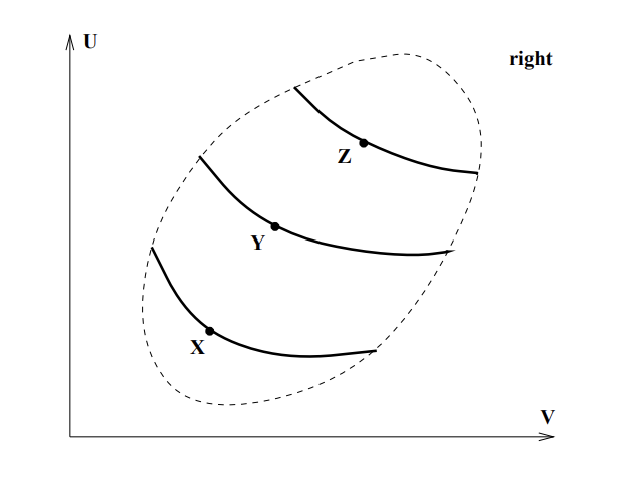
\includegraphics[width=100mm]{fig5.png}
    \end{center}
    \caption{nestの仕方}
    \label{fig:three}
\end{figure}
図3は、nestの仕方を表している図である。このことから、単純系についてのCHが成り立っていることがわかる。\\

\begin{itembox}[l]{\textbf{Thm:$\prec$の包含は存在しない}}
$\prec^{(1)},\prec^{(2)}$を、単純系$\Gamma$の多重スケーリング積における二つの順序関係であるとする。
このとき、任意の$X,Y \in \Gamma$について、
\begin{equation}
    X \prec^{(1)} \Rightarrow \prec^{(2)}
\end{equation}
であるならば、$\prec^{(1)} =\prec^{(2)}$である。
\end{itembox}
\textbf{Prf}\\

\newpage
\section{熱平衡}
単純系の同士の熱的接触について考える。まず、我々は単一単純系のスケールコピーを考えてから、異なる系の積をとる。
このとき肝心なこととしては、熱平衡にある二つの単純系は、一つの新たな単純系とみなせることである。\\

\subsection{熱接触についての仮定}
熱平衡に関する公理を5つ導入する。\\
一つ目の公理は、二つの系を、全系に対して断熱的に、熱平衡状態へと遷移させることができるという意味である。\\
\begin{itembox}[l]{\textbf{T1:熱接触}}
    二つの単純系の状態空間$\Gamma_1,\Gamma_2$が与えられたとき、新たな、熱平衡状態を持つ単純系$\Delta_{12}$が存在する。この系$\Delta_{12}$を、thermal joinという。\\
    $\Delta_{12}$の仕事座標は、$(V_1,V_2)$であり、その範囲はそれらの和の範囲である。また、エネルギー座標についても同様である。記号で表すと、
    \begin{equation}
        \Delta_{12} = \{(U,V_1,V_2):U=U_1+U_2 \quad (U_1,V_1) \in \Gamma_1,(U_2,V_2) \in \Gamma_2\}
    \end{equation}
    である。\\
    ここで、$\Gamma_1 \times \Gamma_2$から$\Delta_{12}$へ向かう断熱操作が存在すると仮定する。すなわち、
    \begin{equation}
        \Gamma_1 \times \Gamma_2 \ni ((U_1,V_1),(U_2,V_2)) \prec ((U_1+U_2,V_1,V_2)) \in \Delta_{12}
    \end{equation}
    である。この操作を、熱平衡化という。
\end{itembox}

\begin{itembox}[l]{\textbf{T2:熱的分離}}
任意の$(U,V_1,V_2) \in \Delta_{12}$について、少なくとも一組の状態$(U_1,V_1)\in \Gamma_1,(U_2,V_2) \in \Gamma_2\quad U=U_1+U_2$が存在し、
\begin{equation}
    \Delta_{12} \ni (U,V_1,V_2) \overset{A}{\sim}((U_1,V_1),(U_2,V_2))\in \Gamma_1 \times \Gamma_2
\end{equation}
を満たす。特に、以下も成立する。
\begin{equation}
    (U,(1-\lambda)V,\lambda V) \overset{A}{\sim}(((1-\lambda)U,(1-\lambda)V),(\lambda U,\lambda V)) \in \Gamma^{(1-\lambda)} \times \Gamma^{\lambda}
\end{equation}
\end{itembox}
以下、状態が等しいことを表す記号をもう一つ導入する。\\
\begin{itembox}[l]{\textbf{Def:熱平衡}}
$X=(U_1,V_1) \quad Y =(U_2,V_2)$に対して、
もし、$((U_1,V_1),(U_2,V_2)) \overset{A}{\sim} (U_1+U_2,V_1,V_2)$であるならば、$((U_1,V_1),(U_2,V_2))$は熱平衡にあるといい、
\begin{equation}
    X \overset{T}{\sim} Y
\end{equation}
と書く。
\end{itembox}
このとき、
\begin{equation}
    X \overset{T}{\sim} Y \Leftrightarrow Y \overset{T}{\sim} X
\end{equation}
および、
\begin{equation}
    X \overset{T}{\sim} X
\end{equation}
は自明である。\\
S3では、実はこの$\overset{T}{\sim}$が同値関係であることをいう。\\

\begin{itembox}[l]{\textbf{S3:熱力学第0法則}}
    \begin{equation}
        X \overset{T}{\sim} Y \quad Y \overset{T}{\sim} Z \Rightarrow X \overset{T}{\sim} Z
    \end{equation}
\end{itembox}
また、$\overset{T}{\sim}$による同値類を、等温線という。\\

\begin{itembox}[l]{\textbf{Thm:熱平衡のスケール不変性}}
    $X,Y$が、二つの単純系の二つの状態であるとし、$\lambda,\mu$が正の定数であるとする。このとき、
    \begin{equation}
        X \overset{T}{\sim} Y \Rightarrow \lambda X \overset{T}{\sim} \mu Y
    \end{equation}
    である。
\end{itembox}
\textbf{Prf}\\
T2により、
\begin{align}
    (X,\lambda X) =((U_X,V_X),(\lambda U_X,\lambda V_X)) \overset{A}{\sim} ((1+\lambda)U_X,V_X,\lambda V_X) 
\end{align}
である。これは、熱平衡の定義から、$X \overset{T}{\sim} \lambda X$であることを意味する。同様に、$Y \overset{T}{\sim} \mu Y$である。よって、T3を用いることにより、
\begin{align}
    \lambda X \overset{T}{\sim} X \overset{T}{\sim} Y \overset{T}{\sim} \mu Y
\end{align}
である。以上より、示された。\hfill\qedsymbol\\

\begin{itembox}[l]{\textbf{Thm:forward sectorの向き}}
すべての単純系のforward sectorは、同じ方向を向いている。
\end{itembox}
\textbf{Prf}\\

\begin{itembox}[l]{\textbf{Thm:エントロピー最大原理}}
    $S$が単純系の状態空間におけるエントロピー関数であるとき、$S$は$U$について上に凸な関数である。\\
    もし、$S_1,S_2$が$\Gamma_1,\Gamma_2$の一貫したエントロピー関数であって、$(U_i,V_i)\in \Gamma_i$であるとき、
    \begin{equation}
        (U_1,V_1) \overset{T}{\sim} (U_2,V_2) 
    \end{equation}
    となるための必要十分条件は、エントロピーの和が$((U_1,V_1),(U_2,V_2))$において最大となることである。すなわち、
    \begin{equation}
        \underset{\text{max}}{S_1(W,V_1)+S_2((U_1+U_2-W),V_2)} =S_1(U_1,V_1)+S_2(U_2,V_2)
    \end{equation}
    である。

\end{itembox}
\textbf{Prf}\\
T1より、
\begin{align}
    (((1-\lambda)U,(1-\lambda)V),(\lambda U',\lambda V)) \prec ((1-\lambda)U+\lambda U',(1-\lambda)V,\lambda V)
\end{align}
である。ここで、$U'' = (1-\lambda)U+\lambda U'$とすると、右辺について、
\begin{align}
    (U'',(1-\lambda)V,\lambda V) &=((1-\lambda)U''+\lambda U'',(1-\lambda)V,\lambda V)\\
    & \overset{A}{\sim} ((1-\lambda)U'',(1-\lambda)V),(\lambda U'',\lambda V) \overset{A}{\sim} (U'',V)
\end{align}
以上より、$    (((1-\lambda)U,(1-\lambda)V),(\lambda U',\lambda V)) \prec (U'',V)$である。\\
エントロピー原理と、エントロピーの加法性から、
\begin{align}
    (1-\lambda)S(U,V)+\lambda S(U',V) \leq S((1-\lambda)U+\lambda U',V)
\end{align}
である。以上より、定理の前半が示された。\\
後半を示す。$(U_1,V_1),(U_2,V_2)$を二つの単純系の状態とする。このとき、T1を用いることにより、
\begin{align}
    ((W,V_1),(U_1+U_2-W,V_2)) \prec (U_1+U_2,V_1,V_2)
\end{align}
である。熱平衡の定義より、
\begin{align}
(U_1+U_2,V_1,V_2) \overset{A}{\sim} ((U_1,V_1),(U_2,V_2)) \Leftrightarrow (U_1,V_1) \overset{T}{\sim} (U_2,V_2)
\end{align}
である。以上より、
\begin{align}
    S_1(W,V_1)+S_2((U_1+U_2-W),V_2) \leq S_1(U_1,V_1)+S_2(U_2,V_2)
\end{align}
である。以上より、示された。\hfill\qedsymbol\\

\begin{itembox}[l]{\textbf{T4:Transversality}}
    $\Gamma$が単純系の状態空間で、$X \in \Gamma$とする。このとき、
    \begin{equation}
    \exists X_0 \overset{T}{\sim} X_1 \quad s.t.\quad  X_0 \prec \prec X \prec \prec X_1
    \end{equation}
    である。
\end{itembox}
すなわち、任意の断熱曲線上の点について、その両側の点を通るような等温曲線が存在するということである。\\
\begin{figure}[H]
    \begin{center}
    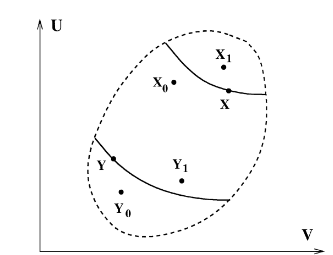
\includegraphics[width=100mm]{fig6a.png}
    \end{center}
    \caption{T4のイメージ}
    \label{fig:four}
\end{figure}

\begin{itembox}[l]{\textbf{T5:普遍的な温度範囲}}
    $\Gamma_1,\Gamma_2$が単純系の状態空間であるとする。このとき、$X \in \Gamma_1$と$V \in \rho (\Gamma_2)$について、$Y \in \Gamma_2$が存在して、
    \begin{equation}
        \rho(Y) =V \quad \text{and} \quad X \overset{T}{\sim} Y
    \end{equation}
    である。
\end{itembox}
これは、

\subsection{複合系の比較原理}
\begin{itembox}[l]{\textbf{Thm:単純系の多重スケーリングコピーにおける比較可能性}}
    $a_1,a_2,\cdots,a_n$が正の実数であるとし、$a_1+\cdots +a_n=a_1'+\cdots+a_m'$であるとする。\\
    このとき、$a_1 \Gamma \times a_2 \Gamma \times \cdots \times a_n \Gamma$と$a_1' \Gamma \times a_2' \Gamma \times \cdots \times a_m' \Gamma$の任意の点は比較可能である。
\end{itembox}
\textbf{Prf}\\
%TODO:あとで書く
\hfill\qedsymbol\\


\subsection{Transversalityの役割}

\newpage
\section{温度とその性質}
温度を導入する。\\
\subsection{エントロピーの微分可能性と温度の存在}
エントロピー関数$S$は、単純系の状態空間$\Gamma$で記述され、上に凸であった。それゆえ、任意の$X \in \Gamma$に対して、$S$の$U$についての左右の微分が存在する。\\
\begin{align}
    \frac{1}{T_+} =\lim_{\epsilon \to 0} \frac{S(U+\epsilon,V)-S(U,V)}{\epsilon}\\
    \frac{1}{T_-} =\lim_{\epsilon \to 0} \frac{S(U,V)-S(U-\epsilon,V)}{\epsilon}
\end{align}
このとき、$T_+,T_-$は、Planckの原理により、有限かつ常に正である。\footnote{有限な理由はtangent planeに関する公理からだと思われる。}\\
これらの関数はそれぞれ、右温度、左温度と呼ばれる。凸性により、
\begin{equation}
    T_-(U_1,V) \leq T_+(U_1,V) \leq T_-(U_2,V) \leq T_+(U_2,V)
\end{equation}
が任意の$U_1<U_2$に対して成立する。\\

\begin{itembox}[l]{\textbf{Lem:断熱曲線上における温度の連続性}}


\end{itembox}
\textbf{Prf}\\
後で書く。\hfill\qedsymbol\\

ここで、熱平衡と温度の関係を考える。\\
エントロピー最大原理により、$X_1=(U_1,V_1),X_2=(U_2,V_2)$に対して、
\begin{equation}
    X_1 \overset{T}{\sim} X_2 \Leftrightarrow S(X_1) +S(X_2) =\underset{W}{\text{max}}\{S(U_1+U_2-W,V_1)+S(W,V_2)\}
\end{equation}
である。ここで、$S$は上に凸であるから、任意の状態空間$\Gamma$上の点$X$に対して、右側温度と左側温度が存在する。ここで、
\begin{equation}
    T(X) = [T_-,T_+]
\end{equation}

により、温度の区間を定義する。このとき、エントロピー最大原理の意味するところは、
\begin{equation}
    X_1 \overset{T}{\sim} X_2 \Leftrightarrow T(X_1)\cap T(X_2) \neq \emptyset
\end{equation}
である。\\
とくに、左右の微係数が等しいとき、
\begin{equation}
    X_1 \overset{T}{\sim} X_2 \Leftrightarrow T(X_1)=T(X_2)
\end{equation}
である。\\
以下の定理で、最後の式が成り立つことが示される。\\

\begin{itembox}[l]{\textbf{Thm:温度の一意性}}

\end{itembox}
\subsection{等温曲線と断熱曲線の幾何}
等温曲線が、途中で途切れることがないことを示す。\\  

\subsection{熱平衡とエントロピーの一意性}
\begin{itembox}[l]{\textbf{Thm:断熱曲線と等温曲線によるエントロピーの一意性}}
    $\prec,\prec^{*}$を、単純系の多重スケーリングコピー上の関係とし、これまで述べた公理を満たすとする。このとき、$\overset{T}{\sim},\overset{T^{*}}{\sim}$を、それぞれ$\prec,\prec^{*}$によって定義される熱平衡関係とする。\\
    このとき、もし、$\prec,\prec^{*}$が$\Gamma$で一致し、$\overset{T}{\sim},\overset{T^{*}}{\sim}$も一致するならば、$\prec,\prec^{*}$は任意の状態空間で一致する。\\
    言い換えると、任意の多重スケーリングコピー上の関係は、断熱曲線及び等温曲線によって定まり、エントロピーは、アフィン変換を除いて一意である。
\end{itembox}
\textbf{Prf}\\


\end{document}